% report.tex
\documentclass{article}
\usepackage{times}
\usepackage{graphicx}
\usepackage{booktabs}
\usepackage{multirow} 
\usepackage{longtable}
\usepackage{hyperref}
%Bold table headings:
\usepackage{array, booktabs}
\usepackage{makecell}
\renewcommand\theadfont{\bfseries}
\usepackage[table]{xcolor}

%Bold captions for images
\usepackage[labelfont=bf]{caption}

\usepackage{float}

\begin{document}

% Title page
\begin{titlepage}
    \vspace*{\stretch{1.0}}
    \begin{center}
        \Large{Udacity Machine Learning Nanodegree Capstone}
        
        \LARGE\textbf{Using deep learning for anomaly detection in geophysical survey}
        
        \vspace{1cm}
        \large\textit{Jiri Vrany}
        
        \normalsize{September, 2017}
    \end{center}
    \vspace*{\stretch{2.0}}
\end{titlepage}


\section{Definition}\label{i.-definition}

\subsection{Project Overview}\label{project-overview}

The usual result of any geophysical survey is a dataset with the
description of features hidden under the Earth surface. Analysis of such
dataset requires a lot of skills and specific knowledge. The precise
analysis takes a long time even for a skilled geophysicist.

On the other hand, there are situations, where we a need to do a quick
survey on site. For example the detection of damaged infrastructure
after an earthquake or flooding. The rescue team needs to be able to do
a quick survey, with the instant result if possible. Some level of
precision can be traded for speed in such situation.

Recent research shows that the methods of computer vision can be used
for analysis of potential field provided by the gravimeter. This
includes the machine learning methods. The potential field model of
gravitation anomaly \cite{salem}
can be visualized as a 2D or 3D image. The final goal, beyond the scope
of this project, is to create a fast but reliable anomaly detection and
classification model.

\subsection{Problem Statement}\label{problem-statement}

Gravity anomaly is the difference between expected and observed gravity
value. The anomaly indicates, that under the earth surface are objects
with different density. The contrast of densities can show us heavy
objects or cavities. Various anomalies generate the various potential
field.

The goal of this project is to explore if the methods of deep learning
can be used to create fast and efficient classifier of the anomaly
type.

\subsection{Metrics}

We used the classification accuracy as a primary evaluation metric. A
classification accuracy is a number of correct predictions from all
predictions made by the model.

For the accuracy computation, We used the algorithm described in
{[}3{]}.

First, compute the correct predictions tensor:

\begin{verbatim}
correct_prediction = tf.equal(tf.argmax(y,1), tf.argmax(y_,1))
\end{verbatim}

Then cast this tensor of booleans to float32 and compute the accuracy as
the mean value of the tensor.

\begin{verbatim}
accuracy = tf.reduce_mean(tf.cast(correct_prediction, tf.float32))
\end{verbatim}

The second method used for analysis of the result was the confusion
matrix. The confusion matrix is often used for visualization of
classification algorithm result. An element of the matrix represents the
number of testing samples classified as a certain class. We can easily
see where the algorithm performs well or where it misclassify some data.

\section{Analysis}\label{ii.-analysis}

\subsection{Data Exploration}\label{data-exploration}

Traditional geophysical surveys do not provide enough data to train the
machine learning models. Either the datasets are small or not available
for public or both.

That is why the artificial dataset with several anomaly types was
created. This dataset is based on the physical models described in \cite{salem}
The real field data do not correspond with the artificial model
directly, but they can be interpolated to the same format with the
gridding process.

The created dataset consists 29992 synthetical models for the area of
size 100x100 meters. The sampling step in measuring is 1 m. Modeled
anomalies are spherical anomaly, vertical cylinder, and horizontal
cylinder.

All anomalies have a random size and random position inside the area.
Each of the models can be represented with 100x100x1 tensor with a known
label.

For each anomaly type, 10000 samples were generated. However, the total
number of samples is slightly lower. The generator script creates the
file name with the sample from the anomaly parameters. And if the script
generates the same random parameters twice, the previous file is simply
overwritten.

The original dataset was split to the testing, validation and training
part. The testing set contains 1000 randomly selected samples and has
been completely taken off the training/evaluation process.

\begin{figure}[!htp]
\centerline{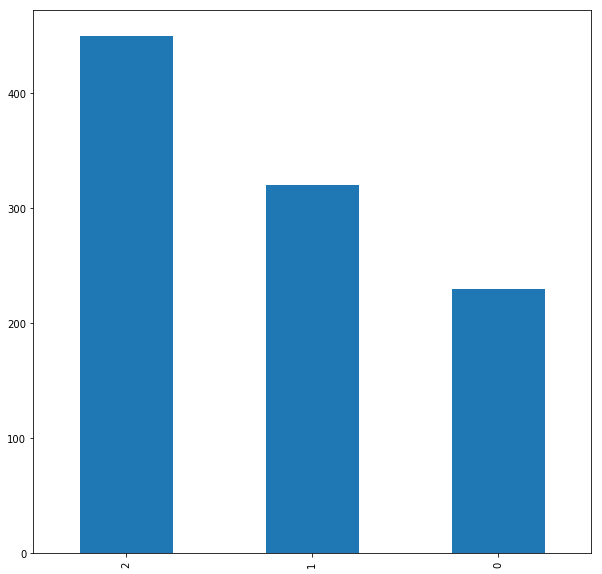
\includegraphics[width=7cm]{img/test_set_frequency.png}}
\renewcommand{\figurename}{Figure}
\caption[Distribution of anomaly type in testing dataset. 0 =
Sphere, 1 = Vertical c., 2 = Horizontal c.]{Distribution of anomaly type in testing dataset. 0 =
Sphere, 1 = Vertical c., 2 = Horizontal c.}
\label{fig:SphericalAnomalyDefinition}
\end{figure}


\subsection{Exploratory
Visualization}\label{exploratory-visualization}

Each anomaly generates specific potential field based on its gravity
effect. This effect is proportional to the density of the anomaly
object.

\begin{figure}[!htp]
\centerline{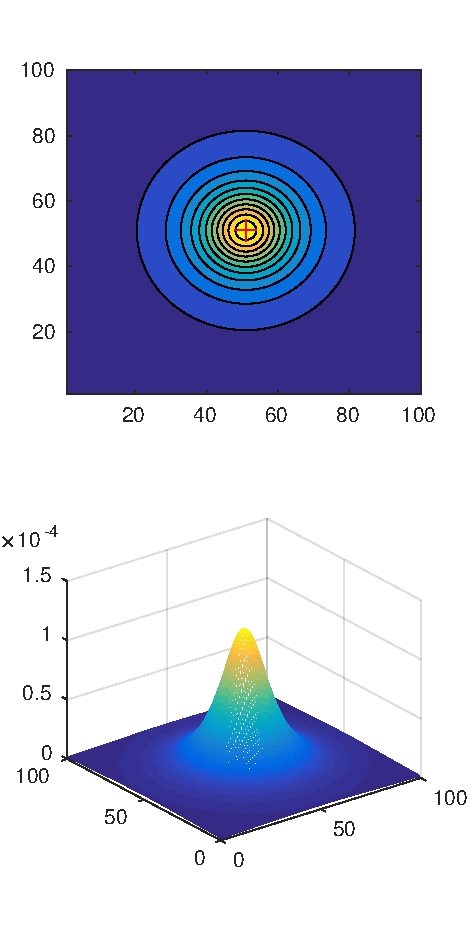
\includegraphics[width=8cm]{img/Sphere_-_density_50_50_15_1000000_5_100_1_100_1.pdf}}
\renewcommand{\figurename}{Figure}
\caption[Input data example - Spherical anomaly]{The example of used input data, spherical anomaly, density contrast $1$ $gcm^{-3}$, radius 5 m, situated in the middle of the area, located 15 m under the surface.}
\label{fig:SphericalAnomalyExample}
\end{figure}

\begin{figure}[!htp]
\centerline{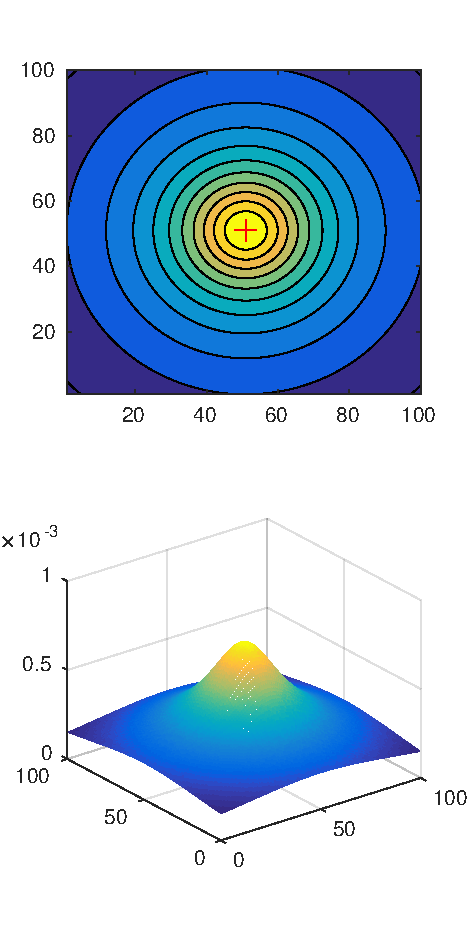
\includegraphics[width=8cm]{img/Vertical_cylinder_50_50_15_1000000_5_100_1_100_1.pdf}}
\renewcommand{\figurename}{Figure}
\caption[Input data example - Vertical cylinder]{A model of vertical cylinder, density contrast $1$ $gcm^{-3}$, radius 5 m, situated in the middle of the area, located 15 m under the surface.}
\label{fig:VerticalAnomalyExample}
\end{figure}

\begin{figure}[!htp]
\centerline{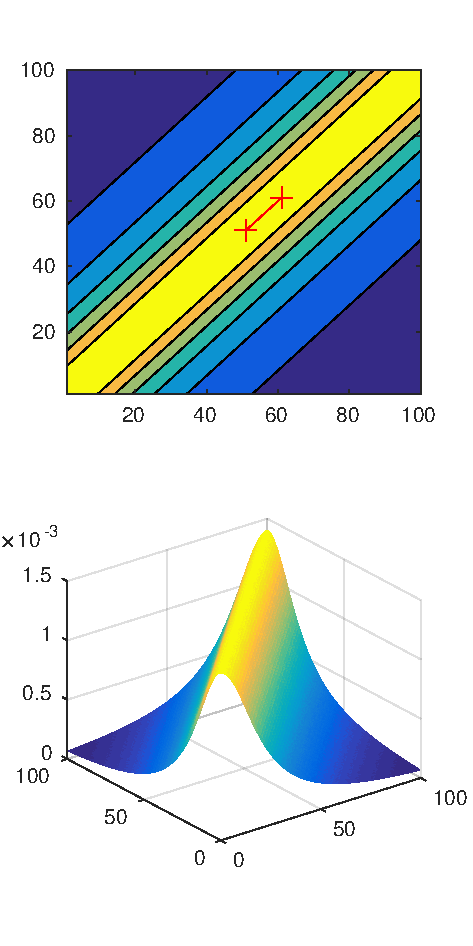
\includegraphics[width=8cm]{img/Horizontal_cylinder_50_50_60_60_15_1000000_5_100_1_100_1.pdf}}
\renewcommand{\figurename}{Figure}
\caption[Input data example - Horizontal cylinder]{A model of horizontal cylinder, density contrast $1$ $gcm^{-3}$, parallel with the surface, running diagonally, radius 5 m, located 15 m under the surface.}
\label{fig:HorizontalAnomalyExample}
\end{figure}

Looking to the examples of each anomaly we can see, that the potential
field for horizontal cylinder has a specific shape, and can be clearly
distinguished from the other two anomalies. On the other hand, the
difference between the sphere and the vertical cylinder is not that
clear. The field generated by the sphere is leaner and more oblong - the
peak is steeper than for the vertical cylinder. With the random size of
anomaly field generated by larger sphere can be easily misclassified as
the field generated by a smaller vertical cylinder. This is the place
where some human or machine expertise is required.

\subsection{Algorithms and
Techniques}\label{algorithms-and-techniques}

The Convolutional Neural Networks (CNN) are considered as a
state-of-the-art in the field image recognition. In many research papers
and real situations, they are reported to work well for finding patterns
in the images and for the image classification. Detail description of
CNN can be found lecture notes of A. Karpathy {[}7{]}

Let's briefly recap that typical CNN is composed of several layers. The
input layer in our case is the potential field represented by a 2D
array. In general, it can be an image in RGB or another format, once
again in form of 2D array. The input layer is connected to several
convolutional layers, typically more than two. In convolutional layer,
we apply set of filters to the input to generate new features. Next, the
output of convolutional layer is used as the input of pooling layer.
Pooling layer contains the activation function and the downsampling
operation.

After several convolution and pooling steps, the fully connected layer
is used for reduction the size of data to a number of classes. One or
more fully connected layers can be used. The final step of the CNN is
the classification layer. In this layer we assign the class belong
probability to the results of the fully connected layer. As for normal
neural network, we use a backpropagation algorithm to adjust the weights
of the neurons in the network and to let the network learn.

The basic implementation of layers, optimization, and neural network
training is available in many open-source libraries such as Tensor Flow,
Torch or Keras. However, there is still a lot of parameters that must be
properly selected and tuned before CNN starts learning efficiently. The
most important parameters tuned in this project were:

\begin{itemize}
\item
  \textbf{The number of hidden layers}. The number of layers is a basic
  parameter of each neural network architecture. It should correspond
  with the number of input parameters, amount of training data, the
  complexity of classification problem and the training algorithm. There
  is no general golden rule but start with the simple network and add
  layers if necessary seems to be a reasonable strategy.
  
\item
  \textbf{Size of convolutional filters}. The size of neuron receptive
  field (or filter size) depends on the type of data that we want to
  classify. If small and local features are important for classification
  of images we should use smaller filters (5x5, 3x3). If larger features
  are more significant larger filters (9x9, 11x11) can be more
  effective. The recent trend is to use more convolutional layers with
  smaller filters because it is more memory efficient. For our data
  larger features are more important, because smaller features in the
  field are mostly caused by residual noise. Therefore larger filters
  should work better.
\item
  \textbf{Minibatch size}. Mini batches are used to reduce the
  computation cost of training. For large dataset is even impossible to
  train the network on the whole dataset. It is reported that smaller
  mini batches help to create a more generalized model and to converge
  faster \cite{minibatch}
\item
  \textbf{Network Optimization method}. The classic method for updating
  network weights is stochastic gradient descent. After 2012 several
  advanced algorithms were introduced, and Adam optimizer
  \cite{adam} seems to be the best one of
  them \cite{gradient-comparsion}. It is able to adapt
  the learning ratio during the training and it is a default optimizer
  in Tensor Flow. It has several parameters for tuning but initial
  learning rate is probably still the most important one.
\item
  \textbf{Dropout}. Dropout is the method used to reduce network
  overfitting introduced in AlexNet paper
  \cite{alexnet}.
  In each training step randomly chosen number of neurons is set to zero
  and this helps the network to learn more robust and general patterns
  in the data. The dropout is typically used on fully connected layers.
  In our architecture, there is one such layer with dropout.
\end{itemize}

\subsection{Benchmark}\label{benchmark}

The results of CNN based classifier were compared with two benchmark
models.

The first model was the simple linear model Wxi+b with softmax layer.
This model was trained on similar dataset as CNN.



\begin{figure}[!htp]
\centerline{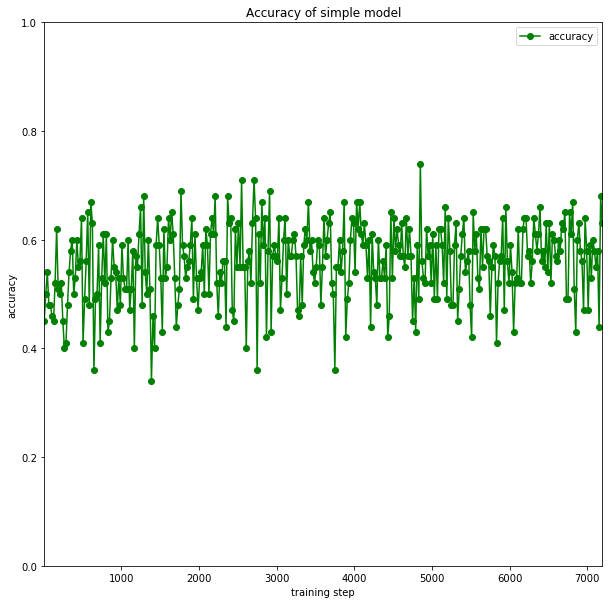
\includegraphics[width=10cm]{img/simple_model_accuracy.png}}
\renewcommand{\figurename}{Figure}
\caption[Accuracy of simple linear model]{Accuracy of simple linear model}
\label{fig:HorizontalAnomalyExample}
\end{figure}


\begin{longtable}[c]{@{}llll@{}}
\toprule
Anomaly type & S & VC & HC\tabularnewline
\midrule
\endhead
Sphere (S) & 71 & 129 & 30\tabularnewline
Vertical cylinder (VC) & 80 & 190 & 50\tabularnewline
Horizontal cylinder (HC) & 180 & 230 & 40\tabularnewline
\bottomrule
\caption[Confusion matrix of simple model]{Cconfusion matrix of simple model.}
\label{tab:ConfusionMatrixSimpleModel}
\end{longtable}

\emph{Table 1. - }

The accuracy of the simple model was oscilating around 50\% during the
training process. However on the training set the simple model failed
and it's result are similar to the random guessing. We can see that the
model makes lot of errors for each anomaly type, not only for the
expected Sphere vs Vertical cylindre.

The second model was originally published in \cite{lenka}
This model was created by classic methods of computer vision such as
edge and line detection. First, the original data are normalized and
thresholded at 9 levels from 0.1 of maximum to 0.9 of maximum to get 9
black and white images. At the level 0.5, the linear structures and
circular regions are searched in the algorithm using the Hough transform
and centroid detection. When objects are detected, the algorithm runs
detection in the other BW images.

The horizontal cylinder is detected, when 2 parallel lines in the same
direction are running through the image. If a circular structure is
detected from level O.9 to O.1 with always the same center, the
hypothesis of other anomaly types is selected. According to the radius
of the circular structure at level 0.5 is calculated the field for these
anomalies. The most similar shape of the field is selected as anomaly
candidate.

\begin{longtable}[c]{@{}lllll@{}}
\toprule
Anomaly type & S & VC & HC & NC\tabularnewline
\midrule
\endhead
Sphere (S) & 175 & 97 & 1 & 47\tabularnewline
Vertical cylinder (VC) & 0 & 295 & 1 & 144\tabularnewline
Horizontal cylinder (HC) & 0 & 0 & 244 & 6\tabularnewline
\bottomrule
\caption[Confusion matrix of benchmark 2 model]{Confusion matrix of benchmark 2 model. NC = not classified.}
\label{tab:ConfusionMatrixBenchmark2}
\end{longtable}


Compared to the machine learning models, there is no need of training
for this model. The model also has one difference - if it has one more
extra ``class'' - not classified. As we can see in the final confusion
table, the model was uncertain about the sphere / vertical cylinder
difference. A lot of vertical cylinders were not classified too.

\section{Methodology}\label{methodology}

\subsection{Data Preprocessing}\label{data-preprocessing}

\paragraph{Noise filtering}\label{noise-filtering}

Each sample in the dataset contains some level of randomly created
noise. This noise was generated to make the artificial data more
realistic. However, the experiments with data during development of
original model \cite{lenka}
proved, that the noise must be filtered out. Without filtering the
algorithm was unable to detect the edges in the data sample at all.
Several methods of filtering were tested and finally, the adaptive
Wiener filter was selected as the preprocessing denoising filter.

After a set of failed attempts to train the network on noised data, we
decide to use the same denoising filter in this project. Denoising will
increase learning algorithm performance and allow to compare the results
of CNN with benchmark algorithm.

\paragraph{Normalization}\label{normalization}

Normalization of data samples is a common preprocessing method for
neural networks. It makes all data values to be in the same range. This
usually improves the convergence of weights and biases in a neural
network. We used the Euclidean (L2) norm for all samples in the dataset.

\paragraph{Dataset augmentation}\label{dataset-augmentation}

We use the horizontal and vertical reflection of original data to create
more training samples for a neural network. Usually, only the horizontal
reflection is used for image data, because it preserves the visual
context of the image. However, for the potential field, we can use the
vertical flip too, because of this only transfer the anomaly to the
different part of the grid.

\subsection{Implementation}\label{implementation}

Preprocessing, simple model and the convolutional neural network were
implemented in Python with Numpy, Scipy, Sklearn, Pandas, and Tensor
Flow libraries.

Our final model has two convolutional layers. Both are using RELU
activation function. The first layer has the convolutional filter of
size 7x7, the depth of the filter is 128. The second layer has the 5x5
filter with depth 256. Both convolutional layers are followed by max
pooling layer. This max pooling layer is using SAME padding and 2x2
kernel. The weights of both layers are initialized by truncated normal
with standard deviation 0.001.

After two convolutional layers are one fully connected layer. This layer
has 1042 nodes and RELU activation function. It is followed by drop out
layer with 40\% dropout rate. The final layer of our model is the
softmax layer.

The model is available in the project repository in two version. First
file initial\_cnn.py contains the initial version, second final\_cnn.py
contains the final tuned model described above.

The data are fed to the model by tensor flow queue. A mini batch of 64
samples is used in the final architecture. After each 10 training steps,
the accuracy is measured on the validation data set.

Preprocessing script transforms the data from the generated txt files to
Tensor Flow Record format. Each file is denoised by wiener filter from
scipy.signal package. Then normalized with L2 norm from sklearn
preprocessing module. Finally, the normalized file is horizontally and
vertically flipped and all three new files are stored in TF Record
format. The preprocessing script is available in the project repository
as preprocess.py.

The generator script for the data was created by Lenka Koskova Triskova
as a part of her research. It is written in Python 2.7 and is available
in the GitHub repository with this report as generator.py.

Simple linear benchmark model is implemented using Tensor Flow and is
available in project repository as simple\_model.py.

\subsection{Refinement}\label{refinement}

The initial architecture of model was similar to the final architecture,
but several parameters were tuned to achieve better results. We started
with 5x5 filter size, the learning rate for optimizer was 0,001 and the
minibatch size 150 which was the biggest size that fit into the memory
of available GPU. The depth of the filter on the first layer was 32 and
64 on the second layer. With this setting, the network did not learn at
all and its precision was close to random guessing.


\begin{figure}[!htp]
\centerline{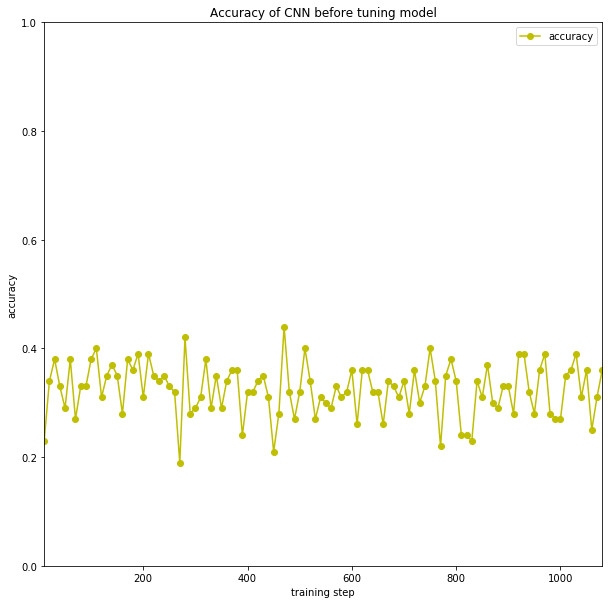
\includegraphics[width=10cm]{img/initial_model_accuracy.png}}
\renewcommand{\figurename}{Figure}
\caption[Accuracy of CNN model before tuning of parameters.]{Accuracy of CNN model before tuning of parameters.}
\label{fig:InitialModelAccuracy}
\end{figure}



We began the refinement of parameters with the increase of the filter
depth to 128 on first and 256 on the second layer. Then increase of
filter size on the first convolutional layer to 7x7, and decrease the
minibatch size to 64. With those settings, the model starts to learn
with good accuracy.

\section{Results}\label{results}

\subsection{Model Evaluation and
Validation}\label{model-evaluation-and-validation}

The final model is stored in the final\_cnn.py file in the project
repository. On previously unseen dataset it was capable to achieve
accuracy between 98-100\% with testing on different parts of the
dataset. During the project preparation and proposal we expected, that
the final model architecture will be more complex and deeper. But this
simple model behaved well.

\begin{figure}[!htp]
\centerline{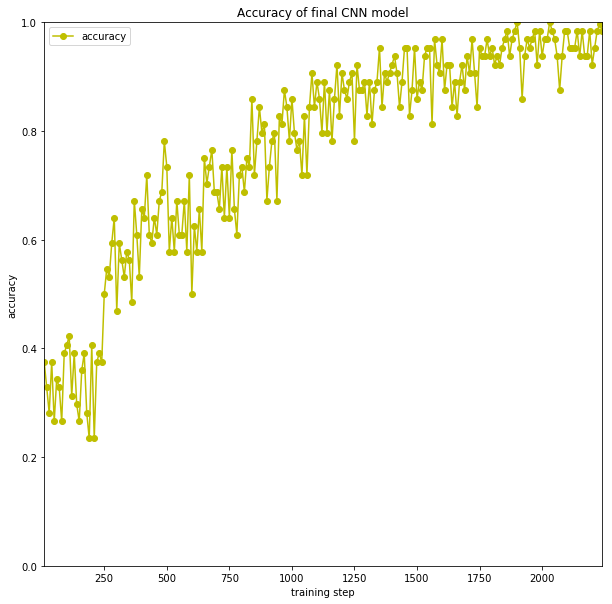
\includegraphics[width=10cm]{img/final_model_accuracy.png}}
\renewcommand{\figurename}{Figure}
\caption[Accuracy of final CNN model.]{Accuracy of final CNN model.}
\label{fig:InitialModelAccuracy}
\end{figure}


During the tuning and debugging process, we trained the model several
times with different training and validation data set. Each time with
the random shuffle of the dataset before the split of training and
validation set. We assume that the model is stable and trustable for
this dataset.

\subsection{Justification}\label{justification}

The final model achieved better results than both benchmarks. This is
important especially in the case of second benchmark model. The CNN is
capable to distinguish between the vertical cylinder and sphere and to
classify all the testing examples. This is a significant improvement of
existing method and it gives a good base for further experiments.

\begin{longtable}[c]{@{}llll@{}}
\toprule
Anomaly type & S & VC & HC\tabularnewline
\midrule
\endhead
Sphere (S) & 220 & 0 & 10\tabularnewline
Vertical cylinder (VC) & 0 & 320 & 0\tabularnewline
Horizontal cylinder (HC) & & 14 & 436\tabularnewline
\bottomrule
\caption[Confusion matrix of final CNN model]{Confusion matrix of final CNN model.}
\label{tab:ConfusionMatrixBenchmark2}
\end{longtable}

\section{Conclusion}\label{conclusion}

\subsection{Reflection}\label{reflection}

In this project, we created convolutional neural network model for
classification of geophysical anomaly. This machine learning model
achieved better results than the benchmark model based on the computer
vision methods.

The new model was trained directly on the potential field data, without
conversion of the dataset to the images. This can be one of the reasons
why the model behaves better. In the transformation of the field of the
image, some information is lost.

It has been proven many times, that the CNN based models perform better
in the field of classification and therefore the results of the project
are as expected. However, in the beginning, we thought that the CNN
model will be capable to learn even from unnormalized noisy data, and
this was not true. We spent a lot of time with different network
architectures and parameters tuning, however without any good results.
The final way to working model was in better preprocessing - the
normalization and denoising turn out to be the right way.

The further research in the geophysical anomaly detection should be
based on CNN models. Stronger classifier opens new possibilities and
further experiments with the more complex dataset with more than one
anomaly or more anomaly types will be possible.

\subsection{Improvement}\label{improvement}

In the beginning of the project we thought about more than three anomaly
classes. But because we have the results of the benchmark model only for
those three it was not necessary to create additional data samples. This
would be the interesting improvement of the project, and it can help to
create the more robust model for the real situations.

This project was proof of concept which turns to the success. Now we can
start to classify more anomalies, but also start to work on the
detection of the anomaly position, the different levels of noise and
other improvements of this basic model.

\begin{thebibliography}{References}
\bibitem{Salem}Salem A.: Multi-deconvolution analysis of potential field data, Journal of Applied Geophysics, 2011, Vol. 74, Issue 2-3, Pages 151-156.
\bibitem{Stanford}S class CS231n: Convolutional Neural Networks for Visual Recognition: A course notes, available online at \href{http://cs231n.github.io/}{http://cs231n.github.io/}.
\bibitem{adam}Diederik P. Kingma, Jimmy Ba: Adam: A Method for Stochastic Optimization, 3rd International Conference for Learning Representations, San Diego, 2015
\bibitem{gradient-comparsion}Sebastian Ruder: An overview of gradient descent optimization algorithms
\bibitem{alexnet}Alex Krizhevsky and Sutskever, Ilya and Hinton, Geoffrey E: ImageNet Classification with Deep Convolutional Neural Networks, Advances in Neural Information Processing Systems 25, 2012
\bibitem{tfmanual}TensorFlow manual: Deep MNIST for Experts, 2017

\end{thebibliography}

\end{document}